\documentclass[11pt,a4paper]{book}
\usepackage[english]{babel}
\usepackage{graphicx}
\usepackage[a4paper,textwidth=16cm,top=2cm,bottom=4cm,left=2.5cm,right=2.5cm]{geometry}

\newcommand{\matlab}[0] {MATLAB\textregistered\ }

\title{\Huge \bf MUSHRAM 1.0\protect\\\vspace{.5cm}
\LARGE User guide}
\author{\Large  Emmanuel \sc{Vincent}\\
Centre for Digital Music\\
Queen Mary, University of London\\
November 2005}
\date{}

\begin{document}

\maketitle

\vfill
 \tableofcontents

\vfill

\chapter{Before you start}
This document is meant to help you use the MUSHRAM interface for MUSHRA listening tests under \matlab\footnote{\matlab is a registered trademark of The MathWorks, Inc.}.

\section{Required knowledge about listening tests}
MUSHRA means ``MUlti Stimulus test with Hidden Reference and Anchor''. This is the recommendation ITU-R BS.1534-1 \cite{ITU03} for the subjective assessment of intermediate quality level of coding systems. In other words, MUSHRA listening tests allow the comparison of \textit{high quality reference sounds} with several \textit{lower quality test sounds}. If the test sounds have a near-transparent quality or if the reference sounds have a low quality, then other types of listening tests should be conducted.\\

You should be familiar with the concepts of MUSHRA listening tests prior to using MUSHRAM. For instance, it is recommended that you read thoroughly the text of the ITU-R recommendation, which can be downloaded for free on the ITU website by registering beforehand on \texttt{http://ecs.itu.ch/cgi-bin/ebookshop}. You should also read other recommendations related to subjective evaluation of audio quality to make sure that MUSHRA listening tests are an appropriate answer to your problem.

\section{Required experience with MATLAB}
MUSHRAM is a set of MATLAB routines. You should be familiar with MATLAB prior to using it. 
\vfill

%%%%%%%%%%%%%%%%%%%%%%%%%%%%%%%%%
\chapter{License and installation}
\section{License and citation}
MUSHRAM is distributed under the terms of the GNU General Public License Version 2. A copy of the license is provided with this distribution. If you use MUSHRAM within an article, a paper, a report or any other work that you wish to publish, please cite it as:\\[.5em]
E.~Vincent, {\it MUSHRAM: A MATLAB interface for MUSHRA listening tests}, 2005,\\
\texttt{http://www.elec.qmul.ac.uk/people/emmanuelv/mushram/}

\section{Download and install}
MUSHRAM can be downloaded at\\[.5em]
\texttt{http://www.elec.qmul.ac.uk/people/emmanuelv/mushram/mushram.zip}\\[.5em]
Once you have downloaded and uncompressed the zip file you should get a directory called \texttt{MUSHRAM} containing the following files
\begin{itemize}
\item MATLAB files \texttt{evaluation\_callbacks.m}, \texttt{evaluation\_gui.m}, \texttt{mushram\_config.m}, \texttt{mushram.m}, \texttt{mushram\_results.m}, \texttt{training\_callbacks.m} and \texttt{training\_gui.m}
\item a license file \texttt{LICENSE.txt}
\item files to generate this user guide \texttt{evaluation\_screenshot.eps}, \texttt{training\_screenshot.eps}, \texttt{user\_guide.pdf}, \texttt{user\_guide.tex}
\end{itemize}
You can then install the program by adding the full path to this directory to MATLAB's path. This can be done for example by typing
\begin{verbatim}
pathtool;
\end{verbatim}
at the MATLAB prompt, clicking on ``Add folder'', selecting the MUSHRAM folder and saving the new path.

\section{Software dependencies}
MUSHRAM depends on the \texttt{sox} package to play WAV sound files under Unix-like platforms (Linux, Mac OS X, Sun). If you are working under such a platform, please make sure you have this package installed too and that the shell command \texttt{play} is working properly.
\vfill

%%%%%%%%%%%%%%%%%%%%%%%%%%%%%%%%%
\chapter{User guide}
\section{Principles of MUSHRA listening tests}
A well-thought listening test starts by a careful \textit{selection of the test material}. MUSHRA listening tests are particularly suited to compare high quality reference sounds with lower quality test sounds. Thus test items where the test sounds have a near-transparent quality or where the reference sounds have a low quality should not be used. All the reference sounds and test sounds must be normalized to the same subjective loudness level. Also the amount of test material must be kept small enough for the subjects to perform the test within a reasonable time. The \textit{selection of the subjects} is also important: for certain types of experiments, the results may vary depending whether the subjects are specialists or not. More detailed guidelines for the selection of test material and subjects are available in \cite{ITU03}.\\

The listening test itself is divided into two successive phases: the \textit{training phase} and the \textit{evaluation phase}.\\

The training phase consists in explaining to the subjects what are the principles of MUSHRA listening tests and what they are expected to do. An example of text that can be distributed to the subjects to this aim is available in \cite{ITU03}. Then each subject listens to all the sounds that he will have to grade in the evaluation phase, paying attention to the different types and levels of impairments that can be heard. During this phase, he can also set the volume of the headphones to a comfortable level, but not too quiet so that impairments still remain perceptible. Recommendations on the volume level are given in \cite{ITU03}.\\

The evaluation phase consists of several successive experiments. The aim of each experiment is to compare a high quality reference sound to several test sounds sorted in random order, including the reference. Each subject is asked to assess the quality of each test sound (relative to the reference and other test sounds) by grading it on a quality scale between 0 and 100. It is not necessary that one test sound be graded 0, however at least one must be graded 100 (because the reference sound is among the test sounds). The test sounds must also include one or several \textit{anchor sounds} computed similarly for all experiments using simple signal processing operations. One of these anchor sounds must be the reference sound low-pass filtered at 3.5~kHz.\\

After all the subjects have graded all the test sounds from all experiments, a \textit{post-screening of the subjects} is performed to reject results produced by subjects that are either not critical enough or too critical. Finally, a \textit{statistical analysis} of the results is conducted. Guidelines about these issues are again provided in \cite{ITU03}.

\section{Important remarks}
The training phase and the design of relevant anchor sounds are essential to obtain consistent gradings between subjects and reproducible results.\\

Without a proper training phase, some subjects tend to be either not critical enough (all sounds graded as good) or too critical (all sounds graded as bad), instead of using the whole grading scale. For instance, if only medium quality test sounds appear in the first experiment and if these test sounds are graded as bad, then low quality test sounds appearing in subsequent experiments will be graded as bad too. Conversely, if low quality test sounds appear in the first experiment and are graded as good, then all the test files in subsequent experiments will be graded as good too. Thus it is important that the subjects listen to all the test sounds during the training phase and identify the largest level of impairment. The consistence of gradings between experiments is also improved by randomizing the order of the experiments.\\

Similarly, the design of relevant anchor sounds is important to evaluate the absolute quality of the test sounds by comparing them to well-defined levels of impairments. Besides the anchor sound consisting of the reference sound low-pass filtered at 3.5 kHz, other anchor sounds should show similar impairment characteristics as the test sounds and be computed with the same simple signal processing operations for all experiments, so as to be easily reproducible.

\section{Configuring the experiments}
\label{sec:config}
In order to setup a MUSHRA listening test using MUSHRAM, type
\begin{verbatim}
mushram_config;
\end{verbatim}
at the MATLAB prompt. A dialog box appears and asks for the number of experiments and the number of files per experiment (including the reference). Then another dialog appears and asks successively for all the file names corresponding to the reference sounds and the test sounds for all experiments. This input information is converted into a configuration file \texttt{mushram\_config.txt} located in the \texttt{MUSHRAM} directory.\\

You can also write the configuration file directly without using the \texttt{mushram\_config} interface. For example, if you want to conduct 2 experiments with 3 files per experiment (including the reference), the configuration file will look like this:\\[.5em]
\begin{tt}
path/reference\_1.wav\\
path/test\_1\_a.wav\\
path/test\_1\_b.wav\\[1em]
path/reference\_2.wav\\
path/test\_2\_a.wav\\
path/test\_2\_b.wav\\[.5em]
\end{tt}
where \texttt{path} is the path to the directory containing the sound files. This path can be specified absolutely or relatively to the \texttt{MUSHRAM} directory or to any other directory present in MATLAB's path.

\section{Starting the experiments}
Once a listening test is configured, each subject can run it by typing
\begin{verbatim}
mushram;
\end{verbatim}
at the MATLAB prompt. The syntax \texttt{mushram('all');} is equivalent. By default, this runs successively two graphical interfaces (one for the training phase and one for the evaluation phase), the order of the experiments is randomized and the order of the test files within each experiment is randomized too.\\
It is possible to run one interface only by typing \texttt{mushram(phase);} where \texttt{phase} equals \texttt{'training'} or \texttt{'evaluation'}. It is also possible to run the experiments in the same order as in the configuration file by typing \texttt{mushram(phase,'no\_random');}, but the order of the test files within each experiment remains randomized.

\section{The training phase}
The training interface is shown in figure \ref{fig:training}. The subject can play the reference sounds or the test sounds (excluding the reference sound) by clicking respectively on the ``Play reference'' or ``Play'' buttons. The button ``Proceed to evaluation'' closes the training interface and opens the evaluation interface.

\begin{figure}[htbp]
\centering
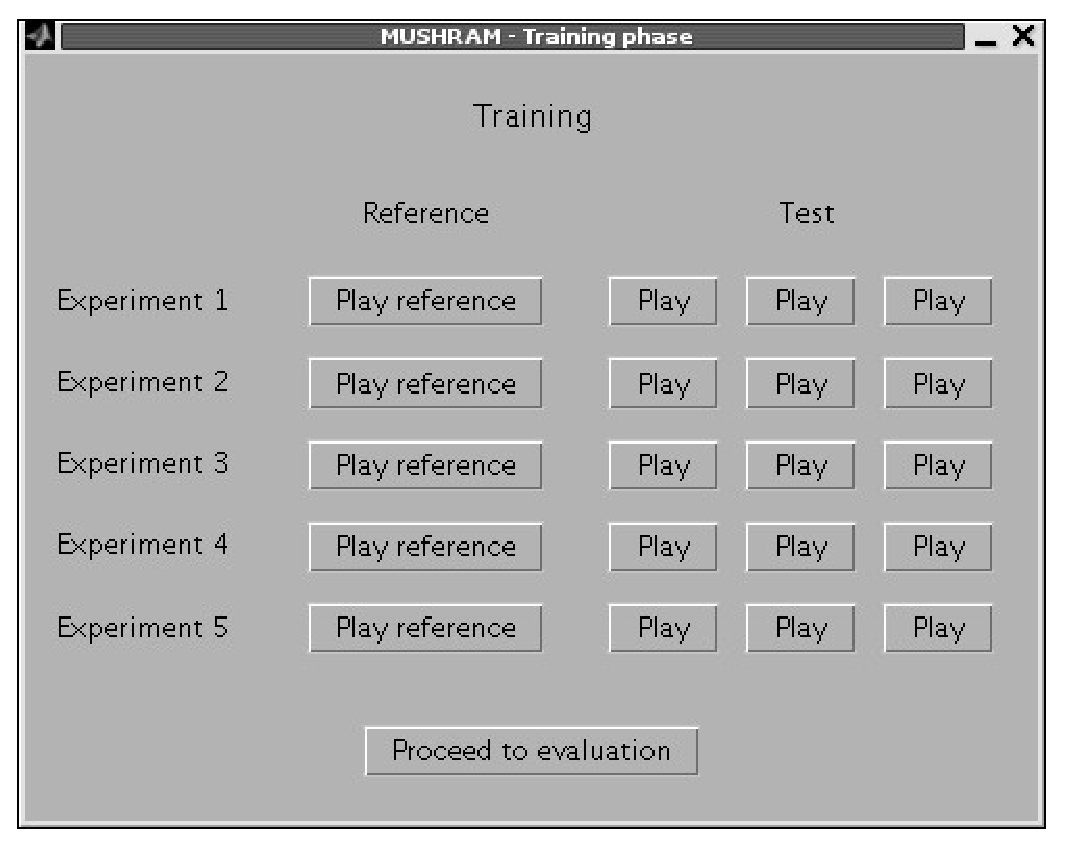
\includegraphics[scale=0.75]{training_screenshot.eps}
\caption{Screenshot of the training interface.}
\label{fig:training}
\end{figure}

\section{The evaluation phase}
The evaluation interface opens a dialog box and asks in which file to save the results. After a file name is entered, the interface for each experiment appears as illustrated in figure \ref{fig:evaluation}. The subject can play the reference sound or the test sounds by clicking respectively on the ``Play reference'' or ``Play'' buttons. Each sound can be graded by moving the corresponding slider and the grading value appears in the corresponding text field. The button ``Save and proceed'' saves the grading values and starts the next experiment.\\

The results are written in the specified file in text format and in the same order as in the configuration file, independently of the order the experiments are run and the test files are presented. More precisely, if the configuration file of section \ref{sec:config} is used, then the content of the results file will be something like this:\\[.5em]
\begin{tt}
100\\
52\\
79\\[1em]
100\\
47\\
69\\[.5em]
\end{tt}
where 100 is the grading corresponding to \texttt{reference\_1.wav}, 52 the grading corresponding to \texttt{test\_1\_a.wav}, \textit{etc}.

\begin{figure}[htbp]
\centering
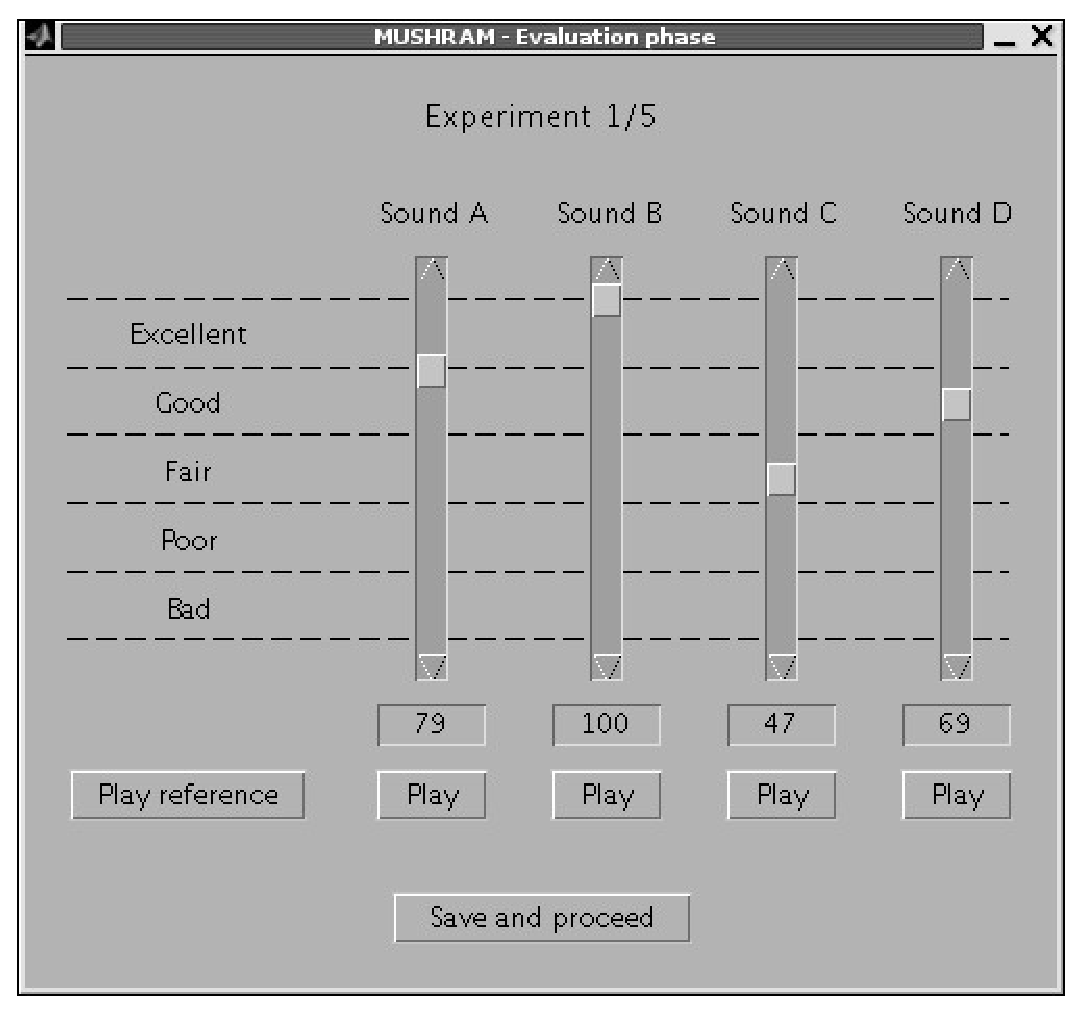
\includegraphics[scale=0.75]{evaluation_screenshot.eps}
\caption{Screenshot of the evaluation interface.}
\label{fig:evaluation}
\end{figure}

\section{Retrieving the results}
The grading values attributed by a given subject can be loaded into MATLAB's workspace by typing
\begin{verbatim}
values=mushram_results(filename);
\end{verbatim}
where \texttt{filename} is the full path to the file where the subject saved the results. The resulting matrix \texttt{values} contains one line per experiment and one column per test file (including the reference). Again experiments and test files are sorted in the same order as in the configuration file.
\vfill

\chapter{Known limitations}
\section{Playing sound files}
Contrary to other software interfaces for MUSHRA listening tests, MUSHRAM cannot switch instantly between two sound files: the sound files have to be played successively. Also MUSHRAM accepts only WAV files currently.

\section{Number of experiments and test files}
The maximal number of experiments and/or test files is limited by the size of the screen. Try increasing the resolution of the screen if you cannot use as many experiments and/or test files as you would like to.

\begin{thebibliography}{WWW}
\bibitem[{ITU}03]{ITU03}
{ITU (International Telecommunication Union)}.
\newblock Recommendation {BS}.1534-1: Method for the subjective assessment of
  intermediate quality levels of coding systems, jan. 2003.\\\texttt{http://www.itu.int/rec/recommendation.asp?type=folders\&parent=R-REC-BS.1534}
\end{thebibliography}
\addcontentsline{toc}{chapter}{Bibliography}

\end{document}